\documentclass[11pt,a4paper]{book}

\usepackage{Appunti_universitari}
\usepackage{soul} % Si', serve solo per una battuta alla linea 854

\begin{document}
\title{Programmazione C++ \\
	\large Riassunto di "The C++ Programming Language" \\
	4a edizione \\
	\textit{Bjarne Stroustrup}}
\author{Jacopo De Angelis}
\maketitle

\pagebreak
\tableofcontents
\pagebreak

\begin{LARGE}
Programma esteso
\end{LARGE}

\begin{itemize}
	\item Introduzione al C++.
	\item Concetti base di programmazione C++
	\begin{itemize}
		\item tipi di dati, puntatori,  reference, scoping
		\item casting,
	\end{itemize}

	\item C++ come linguaggio ad oggetti
	\begin{itemize}
		\item classi, costruttori e distruttori, overloading, metodi friend
		\item inline, constness"
	\end{itemize}
	\item Concetti avanzati di programmazione C++
	\begin{itemize}
		\item overloading degli operatori
		\item metodi virtual, abstract, polimorfismo
		\item ereditarietà
	\end{itemize}
	\item Programmazione generica
	\begin{itemize}
		\item template
		\item iteratori
	\end{itemize}
	\item La libreria Standard (STL)
	\begin{itemize}
		\item Le classi container
		\item Gli algoritmi
		\item Funtori
		\item Multithread
	\end{itemize}
	\item Uso delle librerie esterne
	\begin{itemize}
		\item Librerie statiche
		\item Librerie dinamiche
		\item La libreria OpenMP
	\end{itemize}
	\item I nuovi standard C++11, C++14

	\item Applicazioni GUI
	\begin{itemize}
		\item Ambiente di sviluppo QT Creator
		\item Sviluppo di interfacce grafiche
		\item Gestione degli eventi
		\item Le librerie Qt, QTWidgetscontenuto...
	\end{itemize}
\end{itemize}
\pagebreak

\chapter{Principi base}
\section{Le basi}
C++ è un linguaggio compilato. Il processo di compilazione è unione dei file è il seguente:
\begin{figure}[h!]
	\begin{center}
		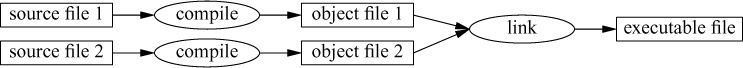
\includegraphics[scale=0.5]{img/001.jpg}
		\caption{Processo di compilazione e unione}
		\label{fig: 001}
	\end{center}
\end{figure}
Il programma è creato per uno specifico sistema operativo. \textbf{C++ è source portable}. Lo standard ISO C++ specifica due entità:
\begin{itemize}
	\item \textbf{Caratteristiche del linguaggio core}: tipi built-in e loop
	\item \textbf{Librerie standard}: container e operazioni I/O
\end{itemize}
\textbf{C++ è un linguaggio fortemente tipizzato e statico}.

\subsection{Hello, World!}
\lstinputlisting[language=C++]{code/001.cpp}\label{code: 001}
Cose che possiamo notare:
\begin{itemize}
	\item \#include <iostream>: include la libreria iostream, ovvero la libreria di I/O
	\item <<: prescrive in inserire il secondo argomento nel primo
	\item //: Commento su singola linea
	\item std::cout: standard output, fa parte del namespace della libreria standard
\end{itemize}

\lstinputlisting[language=C++]{code/002.cpp}\label{code: 002}
Void indica che la funzione non ha valori di ritorno.

\subsection{Tipi, variabili e aritmetica}
Una dichiarazione è una stringa di codice che introduce il nome del programma. É costituita da tipo e nome. I tipi primitivi di C++ sono:
\begin{itemize}
	\item bool
	\item char
	\item int
	\item double
\end{itemize}
In più int, char e double possono anche avere dei modificatori:
\begin{itemize}
	\item long
	\item short
	\item signed
	\item unsigned
\end{itemize}

Le combinazioni sono:
\begin{table}[]
\resizebox{\textwidth}{!}{%
\begin{tabular}{|c|c|c|}
\hline
{\color[HTML]{333333} \textbf{Data type}} & {\color[HTML]{333333} \textbf{Size (bit)}} & {\color[HTML]{333333} \textbf{Range}}                 \\ \hline
short int                                 & 16                                         & -32,768 to 32,767                                     \\ \hline
unsigned short int                        & 16                                         & 0 to 65,535                                           \\ \hline
unsigned int                              & 32                                         & 0 to 4,294,967,295                                    \\ \hline
int                                       & 32                                         & -2,147,483,648 to 2,147,483,647                       \\ \hline
long int                                  & 32                                         & -2,147,483,648 to 2,147,483,647                       \\ \hline
unsigned long int                         & 32                                         & 0 to 4,294,967,295                                    \\ \hline
long long int                             & 64                                         & -(2\textasciicircum{}63) to (2\textasciicircum{}63)-1 \\ \hline
unsigned long long int                    & 64                                         & 0 to 18,446,744,073,709,551,615                       \\ \hline
signed char                               & 8                                          & -128 to 127                                           \\ \hline
unsigned char                             & 8                                          & 0 to 255                                              \\ \hline
float                                     & 32                                         &                                                       \\ \hline
double                                    & 64                                         &                                                       \\ \hline
long double                               & 96                                         &                                                       \\ \hline
wchar\_t                                  & 16 o 32                                    & 1 wide character                                      \\ \hline
\end{tabular}%
}
\end{table}
\emph{sizeof(var)} permette di ottenere la dimensione della variabile.

Aritmetica:
\begin{itemize}
	\item x+y
	\item +x: +1
	\item x–y
	\item –x: -1
	\item x*y
	\item x/y
	\item x\%y: modulo della divisione
	\item
	\item x+=y: x = x+y
	\item ++x: x = x+1
	\item x–=y: x = x-y
	\item ––x: x = x-1
	\item x*=y: x = x*y
	\item x/=y: x = x/y
	\item x\%=y: x = x\%y
\end{itemize}

Comparazione:
\begin{itemize}
	\item x==y: equal
	\item x!=y: not equal
	\item x<y: less than
	\item x>y: greater than
	\item x<=y: less than or equal
	\item x>=y: greater than or equal
\end{itemize}

C++ esegue automaticamente la conversione tra tipi nelle operazioni aritmetiche.

\textbf{Code quality}: mai inizializzare a vuoto se possibile. I tipi definiti dall'utente possono avere un'inizializzazione implicita. \label{Code quality: 001}

\subsection{Costanti}
C++ supporta due tipi di costanti:
\begin{itemize}
	\item const: la varibaile è una costante, non viene modificata. Viene usata generalmente per specificare le interfacce, in questo modo i dati possono essere passati alle funzioni senza che queste possano modificarli
	\item constexpr: la variabile verrà valutata durante la compilazione. Usata soprattutto per specificare le costanti, per permettere il posizionamento dei dati in memoria dove è difficile che vengano corrotti, e per performance
\end{itemize}
\lstinputlisting[language=C++]{code/003.cpp}\label{code: 003}
Affinchè una costante venga valutata dal compilatore, essa deve essere definita come constexpr. Per essere una constexpr, la funzione deve essere molto semplice: deve avere solo il return. Le constexpr possono essere chiamate anche a runtime, in questo caso si comportano normalmente.

Le constexpr sono obbligatorie in certi casi che vedremo poi. In altri casi sono usate per performance. Nel caso un oggetto sia immutabile è necessario pensarci.

\subsection{Puntatori, array e loop}
\subsubsection{Puntatori}
Un array viene dichiarato come \emph{char v[6];} mentre un puntatore \emph{char* p}. Gli array partono da 0. L'arra deve avere una lunghezza costante. Un puntatore può contenere l'indirizzo di un oggetto del tipo appropriato.
\lstinputlisting[language=C++]{code/004.cpp}\label{code: 004}

Possiamo vedere che * indica "contenuto di" mentre \& indica "indirizzo di".
\begin{figure}[h!]
	\begin{center}
		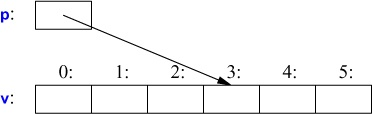
\includegraphics[scale=0.6]{img/002.jpg}
		\caption{Puntatori e indirizzi}
		\label{fig: 002}
	\end{center}
\end{figure}

\subsubsection{Loop}
Ecco due implementazioni del ciclo for:
\lstinputlisting[language=C++]{code/005.cpp}\label{code: 005}
\lstinputlisting[language=C++]{code/006.cpp}\label{code: 006}

Una delle prime cose che notiamo è \emph{auto}: questa parola chiave si occupa di fare inferenza riguardo il contenuto della variabile, serve per non dichiarare esplicitamente che variabile primitiva. Può anche essere utilizzata come tipo di ritorno delle funzioni. Ottima per collegare ad una sola funzione o variabile temporanea più variabili con una notazione generica.

In questi due esempi copiamo il primo vettore nel secondo, ma se volessimo solo dire "incrementa ciò che c'è dentro al vettore ma senza creare una nuova variabile per farlo"? Dovremmo usare un ciclo che implementa dei puntatori e degli indirizzi:
\lstinputlisting[language=C++]{code/007.cpp}\label{code: 007}

In una dichiarazione il suffisso \& significa "reference a". Una "reference" è simile ad un puntatore, eccetto che non ti serve il prefisso * per accedere al valore puntato. In più una reference deve puntare sempre allo stesso oggetto dopo la sua inizializzazione.

Quando usati nelle di dichiarazioni, gli operatori \&, * e [] sono chiamati "operatori di dichiarazione":
\lstinputlisting[language=C++]{code/008.cpp}\label{code: 008}

Un altro tipo di loop è il while:
\lstinputlisting[language=C++]{code/009.cpp}\label{code: 009}

\subsection{Test di verità}
I test di verità, oltre agli operatori ==, != ecc. abbiamo delle funzioni che si occupano di modificare il flusso del programma in base ai valori. Sono if, while e switch:
\lstinputlisting[language=C++]{code/010.cpp}\label{code: 010}
\lstinputlisting[language=C++]{code/011.cpp}\label{code: 011}

\subsection{Tipi definiti dall'utente}
\subsubsection{Strutture}
Il primo modo per costruire un nuovo tipo è, spesso, il riorganizzare i dati in una struttura.
\lstinputlisting[language=C++]{code/012.cpp}\label{code: 012}
Qua possiamo vedere l'implementazione di un vettore tramite \emph{struct} e la sua inizializzazione.

Per inizializzarlo dobbiamo però creare un'apposita funzione:
\lstinputlisting[language=C++]{code/013.cpp}\label{code: 013}
In questo modo la funzione vector\_init ottiene un puntatore alla variabile creata esternamente e il numero di elementi. Il fatto di usare Vector\& serve in modo da ottenere una variabile non locale ma con effetti sulla variabile originale.

L'operatore new alloca memoria per la variabile. Un tipico uso di Vector è questo:
\lstinputlisting[language=C++]{code/014.cpp}\label{code: 014}

Notiamo che questo vettore non è, ovviamente, il vector della libreria standard.

\subsubsection{Classi}
Qua veniamo a conoscenza della differenza tra interfaccia e implementazione di una classe. L'interfaccia è accessibile a tutti, l'implementazione è inaccessibile se non tramite appositi metodi.

La classe è definita da una serie di membri (funzioni, dati o strutture). Questi sono privati, accessibili solo tramite la loro interfaccia pubblica.
\lstinputlisting[language=C++]{code/015.cpp}\label{code: 015}

Una funzione con lo stesso nome della classe è chiamata "costruttore" e ha la funzione di creare la classe con i parametri passati.

\subsubsection{Enumerazioni}
\lstinputlisting[language=C++]{code/016.cpp}\label{code: 016}
Le enumerazioni sono usate per rappresentare un riotto set di valori. Sono usate per rendere il codice più leggibile e meno prono ad errori. Notare che queste enumerazioni sono fortemente tipizzate, ad esempio:
\lstinputlisting[language=C++]{code/017.cpp}\label{code: 017}

Se l'enumerazione non è basata su di una classe ma su di un tipo primitivo basta rimuovere "class".

\subsection{Modularità}
\subsubsection{Compilazione separata}
C++ supporta la compilazione separata dei vari file. Può essere usato per dividere il programma in blocchi di codice semi indipendenti. Questa separazione può essere usata per ridurre il tempo di compilazione richiesto.

Spesso inseriamo le dichiarazioni che specificano l'interfaccia di un modulo in un file denominato header (*.h). Ad esempio possiamo vedere qua prima l'header Vector.h e poi la sua implementazione:
\lstinputlisting[language=C++]{code/018.cpp}\label{code: 018}
Per far sì che il compilatore assicuri la consistenza del codice, anche nella deifnizione viene incluso l'header.

Qua il suo uso:
\lstinputlisting[language=C++]{code/019.cpp}\label{code: 019}

I file possono essere compilati in maniera indipendente, lo schema è più o meno questo:
\begin{figure}[h!]
	\begin{center}
		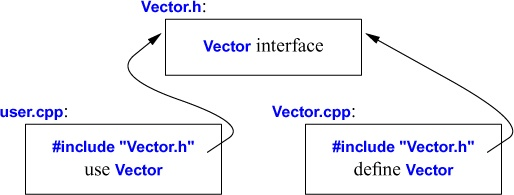
\includegraphics[scale=0.6]{img/003.jpg}
		\caption{Uso dell'header}
		\label{fig: 003}
	\end{center}
\end{figure}

\subsubsection{Namespace}
C++ offre anche i namespace come meccanismo per esprimere alcune dichiarazioni che appartengono allo stesso gruppo senza che vadano in conflitto con altri. Per esempio, potremmo sperimentare con il nostro numero complesso e includerlo nel main in modo che non vada in conflitto con la versione originale:
\lstinputlisting[language=C++]{code/020.cpp}\label{code: 020}

Un modo per accedere alle variabili di altri namespace è \emph{nome\_del\_namespace::funzione/variabile}.Per avere accesso a tutti i nomi della libreria standard possiamo usare la direttiva using, ad esempio \emph{using namespace std;}

\subsection{Gestione degli errori}
\subsubsection{Eccezioni}
Lo schema è il classico try-throw-catch:
\begin{itemize}
	\item Il codice che potrebbe generare un'eccezione viene messo all'interno di un blocco try
	\item L'eccezione viene lanciata con throw
	\item L'eccezione viene gestita da un catch
\end{itemize}

\lstinputlisting[language=C++]{code/021.cpp}\label{code: 021}

\subsubsection{Invarianti}
Prendiamo un esempio classico: cercare di inizializzare un array con un numero negativo. Questa situazione può essere segnalata con un'eccezione della libreria standard, length\_error. In più se il compilatore non riesce ad allocare memoria darà come risposta un'eccezione bad\_alloc. Quindi, il codice diventa:
\lstinputlisting[language=C++]{code/022.cpp}\label{code: 022}

\subsubsection{Asserzioni statiche}
Le eccezioni riportano errori a runtime. Se un errore può essere trovato a tempo di compilazione allora è meglio individuarlo in quel momento. Per farlo possiamo usare le asserzioni statiche. L'importante è che vengano usate con un'espressione costante. Ad esempio:
\lstinputlisting[language=C++]{code/023.cpp}\label{code: 023}

\chapter{Astrazione}
\section{Classi}
Ci sono tre tipi di classi:
\begin{enumerate}
	\item classi concrete
	\item classi astratte
	\item classi nella gerarchia
\end{enumerate}
\subsubsection{Classi concrete}
L'idea è che si comporti esattamente come un tipo built-in. La caratteristiche che definisce un tipo concreto è che la rappresentazione fa parte della definizione.

\paragraph{Un tipo aritmetico}
Questo è un tipo tipo aritmetico definito dall'utente:
\lstinputlisting[language=C++]{code/024.cpp}\label{code: 024}

\paragraph{Container}
Un container è un oggetto che contiene una collezione di elementi, ad esempio un vettore. Pro di Vector: offre controllo di accesso sugli indici e offre una comoda funzione size. Difetto: alloca gli elementi usando new ma non li dealloca mai. C++ offre un'interfaccia per il garbage collector ma non viene usata automaticamente, quindi in certi casi potremmo trovarci a preferire un approccio più preciso. Questo meccanismo è un \emph{destructor}:
\lstinputlisting[language=C++]{code/025.cpp}\label{code: 025}

Il nome del destructor è l'operazione complementare ~ seguita dal nome della classe. É il complemento del costruttore. Il costruttore alloca la memoria nell'heap usando l'operatore new. Il distruttore pulisce usando l'operatore delete.

La tecnica di acquisire le risorse in un costruttore e rilasciarle in un distruttore è nota come \textbf{"Resource Acquisition Is Initialization" o RAII}. Ciò permette di nascondere le operazioni new e delete, separando l'implementazione dall'astrazione.

\paragraph{Inizializzare i container}
Un container esiste per contenere elementi, dobbiamo quindi avere dei metodi comodi per inserirveli. Possiamo creare un vettore con il numero appropriato di elementi e poi aggiungendoli, ma solitamente ci sono modi più eleganti.
Due modi possono essere:
\begin{itemize}
	\item initalize
	\item push\_back(): aggiunge un elemento in fondo alla lista
\end{itemize}

\lstinputlisting[language=C++]{code/026.cpp}\label{code: 026}

Il ciclo for è stato scelto per avere d solo nel suo scope e non occupare memoria dopo. La fine dello stream è decretata da un end-of-file (EOF) o da un errore di formattazione.

\subsubsection{Tipi astratti}
Un tipo astratto isola completamente l'utente dall'implementazione. Per farlo, separiamo l'interfaccia. Poichè non sappiamo niente sulla rappresentazione di un tipo astratto, dobbiamo allocare dello spazio e accedervi tramite puntatori. Prima definiamo una classe container che verrà creata come versione astratta del vettore.
\lstinputlisting[language=C++]{code/027.cpp}\label{code: 027}
La classe è una pura interfaccia ad un container specifico definito più avanti. La parola "\emph{virtual}" significa "potrebbe essere ridefinito più avanti in una classe derivata".

Una classe derivata dalla classe Container offre un'implementazione dell'interfaccia. La curiosa sintassi \emph{=0} dice che la funzione è puramente virtuale, significa che obbligatoriamente deve essere implementata dalla classe derivata.

Non è quindi possibile definire un oggetto che è solo un Container, deve obbligatoriamente implementare \emph{operator[]()} e \emph{size()}. \textbf{Una classe puramente virtuale è detta classe astratta}.
\lstinputlisting[language=C++]{code/028.cpp}\label{code: 028}

Notare come use() utilizzi l'interfaccia Container senza avere alcuna conoscenza della sua implementazione. Utilizza size() e [] senza avere idea di che tipo offra la sua implementazione. \textbf{Una classe che offre un'interfaccia a svariate altre classi è detta di "tipo polimorfico"}.

Come è comune per le classi astratte, Container non ha un costruttore, dopotutto non ha dati da inizializzare. Da un altro punto di vista, Container ha un distruttore e il distruttore è virtuale. Anche questo è normale in quanto solitamente passa un puntatore ad un Container senza conoscere a quale risorsa stia puntando.

Un container che implementa la funzione richiesta dall'interfaccia definita dalla classe astratta potrebbe essere la classe Vector:
\lstinputlisting[language=C++]{code/029.cpp}\label{code: 029}

:public può essere letto come "deriva da" o "è un sottotipo di". La classe Vector\_Container deriva dalla classe Container e questa è detta classe base di Vector\_container. Una terminologia alternativa è classe genitore e classe figlia. Questa proprietà è detta ereditarietà.

I membri operator[]() e size() fanno override dei membri corrispondenti nella classe base Container. Notare come il distruttore fa implicitamente riferimento a quello della classe base.

Per una funzione come \emph{use(Container\&)} usare un Container in completa ignoranza va bene, per altre funzioni dovremo creare un oggetto con il quale operare. Ad esempio:
\lstinputlisting[language=C++]{code/030.cpp}\label{code: 030}

Poichè use() non è a conoscenza dei dettagli di Vector\_container ma conosce solo l'interfaccia Container, funzionerà senza problemi con una diversa implementazione di Container. Ad esempio:
\lstinputlisting[language=C++]{code/031.cpp}\label{code: 031}

\subsection{Funzioni virtuali}
\lstinputlisting[language=C++]{code/032.cpp}\label{code: 032}
Come viene risolte la chiamata a c[i] per operator[]()? Quando h() chiama use() viene chiamato operator[]() di List\_container . Quando g() chiama use(), viene chiamato operator[]() di Vector\_container. Per avere questa risoluzione, un oggetto Container deve contenere l'informazione necessaria per permettere di selezionare la giusta funzione a runtime.

La tecnica classica è che il compulatore converta il nome della funzione virtuale in un indice che verrà aggiunto alla tabella dei puntatori alle funzioni. Questa tabella è chiamata "virtual function table" o semplicemente \emph{vtbl}. Ogni classe ha la sua vtbl che identifica le sue funzioni virtuali. Una rappresentazione grafica è questa:
\begin{figure}[h!]
	\begin{center}
		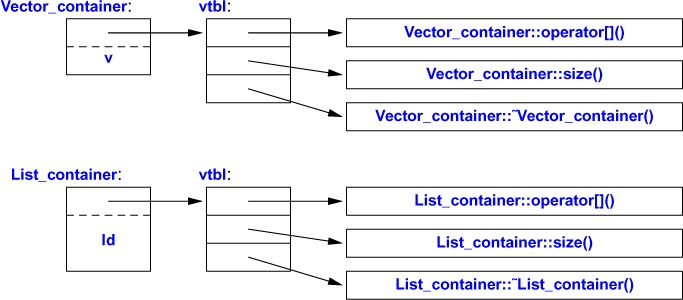
\includegraphics[scale=0.6]{img/004.jpg}
		\caption{vtbl: virtual function table}
		\label{fig: 004}
	\end{center}
\end{figure}

Le funzioni nella vtbl permette agli oggetti di essere usati correttamente anche quando la grandezza dell'oggetto e il tipo di dati sono sconosciuti alla funzione chiamante. All'implementazione della funzione chiamante è richiesta solo la conoscenza del puntatore in una vtbl nel Container e l'indice usato per la funzione virtuale. Questo tipo di chiamata è efficiente quasi quanto quella normale.

\subsection{Gerarchia delle classi}
L'esempio del Container è un caso molto semplice di gerarchia delle classi. Le classi sono ordinate tramite rapporti di derivazione. Ad esempio:
\begin{figure}[h!]
	\begin{center}
		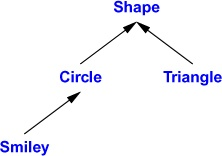
\includegraphics[scale=0.6]{img/005.jpg}
		\caption{Gerarchia delle classi}
		\label{fig: 005}
	\end{center}
\end{figure}
Un esempio è vedere come vengono chiamate e implementate le varie classi:
\lstinputlisting[language=C++]{code/033.cpp}\label{code: 033}
Questa è la definizione della classe base, classe puramente virtuale.

\lstinputlisting[language=C++]{code/034.cpp}\label{code: 034}
Possiamo quindi chiamare in maniera generica la classe astratta shape.

\lstinputlisting[language=C++]{code/035.cpp}\label{code: 035}
Qua vediamo l'implementazione di Circle, classe figlia di Shape.

\lstinputlisting[language=C++]{code/036.cpp}\label{code: 036}
Qua vediamo l'implementazione di Smiley, classe figlia di Circle.

\lstinputlisting[language=C++]{code/037.cpp}\label{code: 037}
Abbiamo finalmente definito la funzione Smiley::draw(). Al suo interno vediamo che chiamiamo la classe genitore Circle come primo passaggio.

Vediamo anche che Smiley fa un override del distruttore della classe genitore. Un distruttore virtuale è essenziale per una classe astratta perchè un oggetto di una classe derivata è solitamente manipolato tramite la sua interfaccia offerta dalla classe astratta. In particolare potrebbe decidere ci cancellare il puntatore alla classe base. Quindi, il meccanismo di chiamata alla funzione virtuale assicura che il distruttore corretto venga chiamato.

Una gerarchia di classi offre due benefici:
\begin{itemize}
	\item Ereditarietà dell'interfaccia: un oggetto di una classe derivata può essere usato per qualunque oggetto venga richiesto. In quesot modo la classe base offre un'interfaccia alla classe derivata.
	\item La classe base offre una funzione o un dato che semplifica l'implementazione.
\end{itemize}

Le classi concrete sono usate esattamente come i tipi built in. Le classi in gerarchie vengono allocate tramite new e vi accediamo tramite puntatori o riferimenti. Per esempio consideriamo una funzione che legge dei dati che descrivono una forma da un input stream e costruisce l'appropriato oggetto Shape:
\lstinputlisting[language=C++]{code/038.cpp}\label{code: 038}
\lstinputlisting[language=C++]{code/039.cpp}\label{code: 039}

Ovviamente questo caso è estremamente semplificato. Ad esempio potremmo notare che il proprietario di un puntatore a Shape potrebbe non cancellarlo, in questo caso un puntatore libero potrebbe essere rischioso. Sarebbe quindi utile rutirnare un unique\_ptr invece di un puntatore normale e immagazzinare il puntatore unico nel container:
\lstinputlisting[language=C++]{code/040.cpp}\label{code: 040}

Ora l'oggetto è posseduto tramite il puntatore unico che verrà cancellato quando non sarà più utile, ovvero quando si uscirà dallo scope che l'ha creato. Per questa nuova versione dobbiamo implementare nuove versioni di \emph{draw\_all()} e \emph{rotate\_all()} che accettano un \emph{vector<unique\_ptr<Shape>>}. Ci sono alternative al dover scrivere tutto che vedremo poi.

\section{Copia e sposta}
Copiare un oggetto complesso significa farne una copia 1 a 1 tramite funzioni ben definite. Se si usasse il semplice simbolo si assegnazione non sarebbe copiato il valore ma il puntatore alla risorsa.

\subsection{Copia}
La copia è definita da due membri: un costruttore di copia e un assegnatore:
\lstinputlisting[language=C++]{code/041.cpp}\label{code: 041}

\subsection{Sposta}
\lstinputlisting[language=C++]{code/042.cpp}\label{code: 042}
Invece di dover copiare ogni signolo valore possiamo copiare il riferimento ai vettori e concatenarli, in questo modo non dobbiamo sprecare risorse aggiuntive.

\& è detto lvalue che più o meno è intendibile come "ciò che andrebbe a sinistra di un assegnamento" mentre \&\& è detto rvalue ovvero "ciò che andrebbe a destra di un assegnamento"

\subsection{Gestione delle risorse}
Offrendo costruttore, copia, spostamento e distruzione, un programma offre una gestione completa della vita di una risorsa.

\section{Template}
Quando qualcuno vuole un vettore non per forza è di double. Usiamo i template per descrivere concetti che è meglio tenere altamente generici.

\subsection{Tipi parametrizzati}
\lstinputlisting[language=C++]{code/043.cpp}\label{code: 043}
Il prefisso template<typename T> rende T un parametro della dichiarazione. É il corrispettivo in C++ di "per ogni T".
I membri della funzione possono essere definiti similarmente:
\lstinputlisting[language=C++]{code/044.cpp}\label{code: 044}

Date queste definizioni possiamo creare ora un vettore così:
\lstinputlisting[language=C++]{code/045.cpp}\label{code: 045}
E così lo possiamo usare:
\lstinputlisting[language=C++]{code/046.cpp}\label{code: 046}

Se vogliamo dare la possibilità di usare un ciclo loop dobbiamo dare un inizio e una fine adatti:
\lstinputlisting[language=C++]{code/047.cpp}\label{code: 047}
Date queste definizioni possiamo scrivere:
\lstinputlisting[language=C++]{code/048.cpp}\label{code: 048}

\subsection{Funzioni template}
Possiamo scrivere comodamente funzioni con i template. Vediamo la parola chiave auto, usata proprio per inferire automaticamente il tipo di x:
\lstinputlisting[language=C++]{code/049.cpp}\label{code: 049}

\subsection{Funzioni oggetto}
Vengono chiamati anche funtori e sono oggetti che possono essere chiamati come funzioni. Perchè? Per programmare funzionalmente.
\lstinputlisting[language=C++]{code/050.cpp}\label{code: 050}
Ad esempio questa funzione chiamata operator() implementa l'operatore (). Possiamo definire variabili di tipo Less\_then tipo:
\lstinputlisting[language=C++]{code/051.cpp}\label{code: 051}

Possiamo chiamare questi oggetti esattamente come chiamiamo le funzioni:
\lstinputlisting[language=C++]{code/052.cpp}\label{code: 052}

\subsection{Template variabile}
Un template che può prendere un numero imprecisato di argomenti è detto "variadic template". Ad esempio:
\lstinputlisting[language=C++]{code/053.cpp}\label{code: 053}

La chiave è separare il primo argomento dal resto e trattarli in maniera ricorsiva.\footnote{Prolog FTW}

\subsection{Alias}
É molto comunque per i template dare "un secondo nome" alle variabili in modo da rendere più comprensibile il corpo della funzione. Ad esempio:
\lstinputlisting[language=C++]{code/054.cpp}\label{code: 054}

\chapter{Contenitori e algoritmi}
\section{Librerie}
\subsection{Headers e namespace della libreria standard}
Ogni libreria standard è offerta tramite qualche header standardizzato, ad esempio:
\begin{itemize}
	\item \#include<string>
	\item \#include<list>
\end{itemize}
La libreria standard è definita all'interno del namespace \emph{std}. Per usare le sue libreria possiamo usare il prefisso \emph{std::}.
\lstinputlisting[language=C++]{code/055.cpp}\label{code: 055}
Ad esempio, per permettere l'utilizzo delle stringhe, all'inizio del file dobbiamo inserire:
\lstinputlisting[language=C++]{code/056.cpp}\label{code: 056}
Generalmente è una pessima scelta includere ogni nome da un namespace.
\begin{figure}[h!]
	\begin{center}
		
\includegraphics[scale=0.6]{img/006.jpg}
		\caption{Lista ridotta degli header standard}
		\label{fig: 006}
	\end{center}
\end{figure}

\begin{figure}[h!]
	\begin{center}
		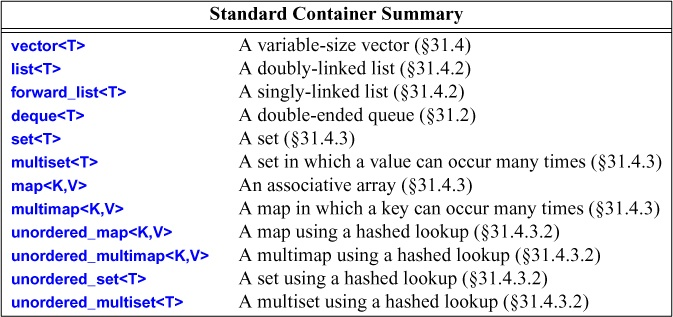
\includegraphics[scale=0.6]{img/007.jpg}
		\caption{Container}
		\label{fig: 007}
	\end{center}
\end{figure}

\chapter{Funzioni base}
\section{Tipi e dichiarazioni}
Per massimizzare la portabilità del codice è saggio essere espliciti in cosa è definito di base e cosa nell'implementazione corrente. Utilizzare solo tipi definiti dallo standard è il prezzo da pagare per la portabilità del codice. Un tipico esempio è di presentare tutte le dipendenze basate sull'hardware in forma di costanti e definire i timi negli header. Per supportare queste tecniche la libreria standard offre \emph{numeric\_limits}. Molti controlli sulle feature derivanti dall'implementazione può essere fatta tramite asserzioni statiche. Ad esempio
\lstinputlisting[language=C++]{code/057.cpp}\label{code: 057}
I comportamenti non definiti sono peggiori, in quanto possono comportare in modi non desiderati. Ad esempio:
\lstinputlisting[language=C++]{code/058.cpp}\label{code: 058}
L'esito più prevedibile è che si vada a sovrascrivere dei dati in aree di memoria non appartenenti all'array.

\subsection{Implementazione}
Un'implementazione di C++ può essere hostata o essere a sè stante. Un'implementazione hostata include tutte le librerie standard. Un'implementazione a sè stante può offrire meno librerie standard finchè le seguenti sono offerte:
\begin{figure}[h!]
	\begin{center}
		
\includegraphics[scale=0.6]{img/008.jpg}
		\caption{Librerie obbligatorie}
		\label{fig: 008}
	\end{center}
\end{figure}

Le implementazioni freestanding sono pensate per codice che possa girare con il minimo delle risorse necessarie.

\subsection{Caratteri di base}
Il set di base si basa su ASCII-7. Per estenderlo un ambiente può mappare il set esteso in più modi, ad esempio usando nomi universali.

\section{Tipi}
\subsection{Tipi fondamentali}
\begin{itemize}
	\item booleani (bool)
	\item Caratteri (char, wchar\_t)
	\item Interi (int, short, long, long int, long long...)
	\item decimali (float, double, long double)
	\item void (assenza di informazione)
\end{itemize}
Da qua si possono costruire altri tipi come:
\begin{itemize}
	\item puntatori (int*)
	\item Array (char[])
	\item riferimenti (double\& e vettori<int>\&\&)
\end{itemize}
In può si possono definire tipi definiti dall'utente:
\begin{itemize}
	\item strutture dati e classi
	\item enumerazioni
\end{itemize}

\subsection{Caratteri}
\begin{itemize}
	\item char: 8 bit
	\item signed char: come har ma può contenere valori positivi e negativi
	\item unsigned char: come char ma garantisce il suo essere senza segno
	\item wchar\_t: offre set estesi come unicode e la sua grandezza è derivante dalla sicurezza
	\item char16\_t: UTF-16
	\item char32\_t: UTF-32
\end{itemize}

\begin{figure}[h!]
	\begin{center}
		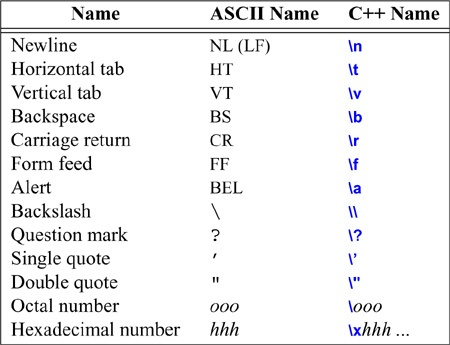
\includegraphics[scale=0.6]{img/009.jpg}
		\caption{Caratteri speciali}
		\label{fig: 009}
	\end{center}
\end{figure}

\subsection{Integrali}
Possono essere decimali, ottali o esadecimali. Se inizia con 0x allora è un esadecimale, se inizia solo con 0 è un ottale.
\begin{figure}[h!]
	\begin{center}
		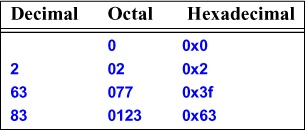
\includegraphics[scale=0.6]{img/010.jpg}
		\caption{Tipi di intero}
		\label{fig: 010}
	\end{center}
\end{figure}

I numeri vengono distinti in base a forma, valore e suffisso:
% Please add the following required packages to your document preamble:
% \usepackage{graphicx}
\begin{table}[]
\resizebox{\textwidth}{!}{%
\begin{tabular}{|c|c|c|l|}
\hline
\textbf{Forma} & \textbf{Valore} & \textbf{Suffisso}                                                                 & \multicolumn{1}{c|}{\textbf{Contenitori adatti}}                                                                                  \\ \hline
               & numero          &                                                                                   & int, long int, long long int                                                                                                      \\ \hline
0, 0x          & numero          &                                                                                   & \begin{tabular}[c]{@{}l@{}}int, unsigned int, long int,\\ unsigned long int, long long int,\\ unsigned long long int\end{tabular} \\ \hline
               & numero          & u, U                                                                              & \begin{tabular}[c]{@{}l@{}}unsigned int, unsigned long int,\\ unsigned long long int\end{tabular}                                 \\ \hline
               & numero          & l, L                                                                              & long int, long long int                                                                                                           \\ \hline
0, 0x          & numero          & l, L                                                                              & \begin{tabular}[c]{@{}l@{}}long int, unsigned long int,\\ long long int, \\ unsigned long long int\end{tabular}                   \\ \hline
               & numero          & \begin{tabular}[c]{@{}c@{}}ul, lu, uL, Lu, Ul, \\ lU, UL, LU\end{tabular}         & \begin{tabular}[c]{@{}l@{}}unsigned long int, \\ unsigned long long int\end{tabular}                                              \\ \hline
               & numero          & ll, LL                                                                            & long long int                                                                                                                     \\ \hline
0, 0x          & numero          & ll, LL                                                                            & \begin{tabular}[c]{@{}l@{}}long long int, \\ unsigned long long int\end{tabular}                                                  \\ \hline
               & numero          & \begin{tabular}[c]{@{}c@{}}llu, llU, ull, Ull, \\ LLu, LLU, uLL, ULL\end{tabular} & unsigned long long int                                                                                                            \\ \hline
\end{tabular}%
}
\end{table}

\subsection{Dimensioni}
Alcuni tipi fondamentali di C++, ad esempio int, sono basati sull'implementazione hardware del sistema. Cosa vuol dire ciò? Che se vuoi fare un sistema portabile bisogna prendersi particolarmente cura di questi piccoli dettagli in modo da non generare problemi.

Limitare l'impatto delle caratteristiche basate sull'implementazione è semplice, limitare l'impatto di caratteristiche basate sull'hardware è decisamente più difficile. Usare le librerie standard quando possibile è sempre un'ottima strategia.

La ragione per l'implementare più tipi di intero e più tipi di float è proprio questa, il dare agli sviluppatori più agio. Ci sono pochi assiomi riguardo le dimensioni:
\begin{itemize}
	\item 1 \equiv sizeof(char) \leq sizeof(short) \leq sizeof(int) \leq sizeof(long) \leq sizeof(long long)
	\item 1 \leq sizeof(bool) \leq sizeof(long)
	\item sizeof(char) \leq sizeof(wchar\_t) \leq sizeof(long)
	\item sizeof(float) \leq sizeof(double) \leq sizeof(long double)
	\item sizeof(N) \equiv sizeof(signed N) \equiv sizeof(unsigned N)
\end{itemize}
Dove N può essere char, short, int, long, long long. In più è garantito che char ha \textbf{minimo} 8 bit, short 16, long 32.

Alcune implementazioni possono essere trovate tramite un semplice sizeof, altrimenti altre possono essere trovate in  <limits>. Ad esempio:
\lstinputlisting[language=C++]{code/059.cpp}\label{code: 059}
Le funzioni in <limits> sono constexpr, quindi possono essere usate senza overhead a runtime.
Se si ha bisogno di tipi particolari si può includere la libreria <cstdint> che include, ad esempio:
\lstinputlisting[language=C++]{code/060.cpp}\label{code: 060}

L'header standard <cstddef> definisce un alias usato molto nelle librerie standard e nel codice utente: size\_t. É un tipo implementato di unsigned int che può contenere la grandezza in byte di qualsiasi oggetto. Quindi è usato quando si vuole avere la grandezza di un oggetto. Ad esempio:
\lstinputlisting[language=C++]{code/061.cpp}\label{code: 061} 

\subsection{Allineamento}\label{par: Allineamento}
L'allineamento dei dati è come i dati vengono disposti in memoria. In certi casi questo dettaglio può permettere di risparmiare molto spazio, ad esempio nelle struct. 

Per fare un esempio:
\lstinputlisting[language=C++]{code/062.cpp}\label{code: 062}
\begin{figure}[h!]
	\begin{center}
		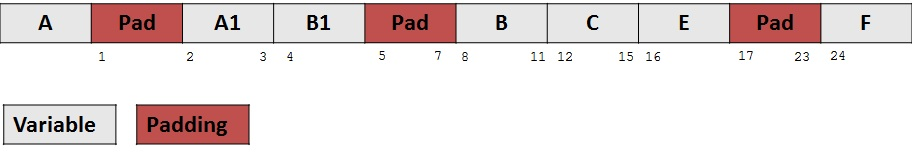
\includegraphics[scale=0.4]{img/011.jpg}
		\caption{Struct "non efficiente"}
		\label{fig: 011}
	\end{center}
\end{figure}
\lstinputlisting[language=C++]{code/062.cpp}\label{code: 063}
\begin{figure}[h!]
	\begin{center}
		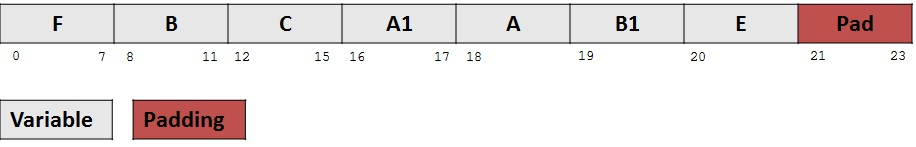
\includegraphics[scale=0.4]{img/012.jpg}
		\caption{Struct "efficiente"}
		\label{fig: 012}
	\end{center}
\end{figure}

La maggior parte delle volte questa cosa non interessa minimamente, si può programmare per anni senza nemmeno pensarci.

L'operatore alignof() può ritornare l'allineamento di un'espressione. Ad esempio:

\section{Dichiarazione}
Deve esserci sempre al massimo una dichiarazione per nome in C. Nel caso ci siano variabili derivanti da librerie esterne ci si può riferire con \emph{extern}.

\subsection{La struttura di una dichiarazione}
\begin{figure}[h!]
	\begin{center}
		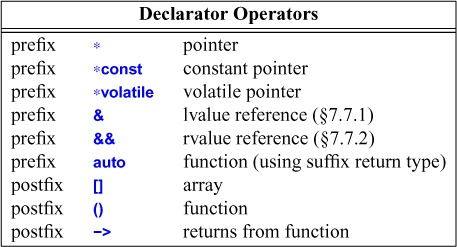
\includegraphics[scale=0.6]{img/013.jpg}
		\caption{Operatori di dichiarazione}
		\label{fig: 013}
	\end{center}
\end{figure}

Le dichiarazioni possono essere fatte in cinque blocchi:
\begin{enumerate}
	\item prefisso opzionale (static o virtual)
	\item tipo base
	\item dichiaratore opzionale che include un nome (ad esempio p[8], n, *)
	\item Suffisso opzionale per le funzioni (const, noexcept)
	\item Inizializzatore opzionale ocorpo di funzione
\end{enumerate}

\subsection{Naming convention}
\subsubsection{File}
\begin{itemize}
	\item .cpp è l'estensione di C++, .c di C e gli header sono .h
	\item Per i file sorente usare file.cpp. Per gli header riferiti usare file.h. Si può anche usare file-impl.h per la dichiarazione di classi che non sono accessibili all'esterno del modulo. Se il file intero dichiara solo simboli interni al modulo, allora -impl è omesso
	\item usare il suffisso -doc.h per i file che contengono solo documentazione di Doxygen
	\item Per C++ cercare di dare al file lo stesso nome della classe che contengono. I file sono tutti all-lowercase
	\item Cercare di evitare classi con lo stesso nome ma in posti differenti
\end{itemize}

\subsubsection{Guideline comuni tra C e C++}
\begin{itemize}
	\item Le macro per il preprocessore sono all-uppercase
	\item i nomi includono le guardie come GMX\_DIRNAME\_HEADERNAME\_H
	\item i boolean hanno sempre prefisso b, seguiti da PascalCase
	\item le variabili enum hanno sempre prefisso e. Generalmente per enumerazioni usate tra più librerie la e è seguita da un altro prefisso, generalmente all-lowercase, per evitare coincidenze (ad esempio epbcNONE).
	\item  Evitare abbreviazioni non comuni
	\item Se si usano acronimi seguire la policy di Microsoft:
	\begin{itemize}
		\item Due lettere: all-uppercase
		\item Tre o più lettere: Normalcase. Nel caso la prima lettera sia generalmente minuscola nell'uso dell'acronimo, allora usare all-lowercase
	\end{itemize}
\end{itemize}

\subsubsection{Codice}
\begin{itemize}
	\item PascalCase per classi, struct e typedef
	\item camelCase per funzioni e variabili
	\item si può usare un nome lo snake\_case per variabili che sono fortemente rassomiglianti dei corrispettivi nella libreria standard-
	\item Le interfacce hanno suffisso Interface
	\item Le classi astratte hanno prefisso Abstract
	\item Per variabili associate ad un oggetto ha un \_ finale
	\item Gli accessori per una variabile foo\_ sono chiamati foo() e setFoo()
	\item Le variabili globali hanno prefisso g\_
	\item Le variabili statiche hanno prefisso s\_
	\item Le costanti globali hanno prefisso c\_
\end{itemize}

\subsection{Parole chiave}
\begin{figure}[h!]
	\begin{center}
		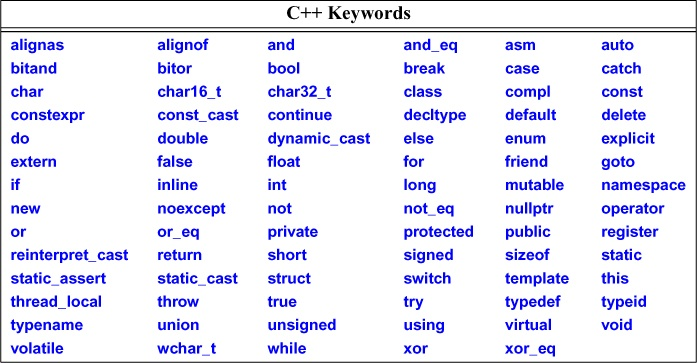
\includegraphics[scale=0.6]{img/014.jpg}
		\caption{Parole chiave}
		\label{fig: 014}
	\end{center}
\end{figure}

\subsection{auto e decltype()}
Solitamente usiamo auto se vogliamo che l'interprete inferisca automaticamente il tipo del dato. In certi casi vogliamo solo dedurne il tipo senza inizializzare una variabile. Quindi possiamo usare decltype(expr) è il tipo di expr. Ad esempio, se sommiamo due matrici di tipo diverso, quale sarà il risultato? Con decltype possiamo saperlo.
\lstinputlisting[language=C++]{code/065.cpp}\label{code: 065}
Quindi:
\begin{itemize}
	\item auto: lo usiamo per inferire il tipo della variaile dal dato
	\item decltype: lo usiamo solo per conoscere il tipo di una funzione o di una variabile
\end{itemize}

Questi due strumenti sono importantissimi per quanto riguarda la programmazione generica.

\subsection{Scope}
\begin{itemize}
	\item \textbf{Local scope}
	\item \textbf{Class scope}
	\item \textbf{Namespace scope}
	\item \textbf{Global scope}
	\item \textbf{Statement scope}
	\item \textbf{Function scope}
\end{itemize}

\subsection{Inizializzazione}
Può essere fatta in più modi:
\begin{itemize}
	\item Tramite assegnamento
	\item Tramite lista di valori
	\item Tramite graffe (rischio di narrowing, ovvero di arrotondamento se necessario)
\end{itemize}
\lstinputlisting[language=C++]{code/066.cpp}\label{code: 066}

Quando inizializziamo dobbiamo considerare due fattori:
\begin{itemize}
	\item il tipo dell'oggetto
	\item il tipo di inizializzazione
\end{itemize}
\lstinputlisting[language=C++]{code/067.cpp}\label{code: 067}
Ad esempio usando l'inizializzatore {} riduciamo il rischio di conversioni
\lstinputlisting[language=C++]{code/068.cpp}\label{code: 068}
Quando usiamo auto interviene solo il tipo dell'inizializzatore, quindi possiamo usare tranquillamente =
\lstinputlisting[language=C++]{code/069.cpp}\label{code: 069}
In effetti, possiamo sfruttare a nostro vantaggio = con auto, poichè l'inizializzatore {} potrebbe creare sorprese inaspettate
\lstinputlisting[language=C++]{code/070.cpp}\label{code: 070}
Il che è abbastanza logico, basti pensare che
\lstinputlisting[language=C++]{code/071.cpp}\label{code: 071}

\section{Oggetti e valori}
\subsection{Durata degli oggetti}
\begin{itemize}
	\item Automatica: a meno che un programmatore specifichi altrimenti, un oggetto dichiarato in una funzione è creato con la sua definizione e distrutto quando il suo nome esce dallo scope.
	\item Statica: gli oggetti dichiarati globalmente o in un namespace e i valori \emph{static} dichiarati in funzioni o in classi sono creati e inizializzati solo una volta e vivono fino al termine del programma. Possono creare problemi in multithread, per questo bisogna implementare un sistema di lock
	\item Free store: usando new e delete possiamo creare oggetti la cui gestione è esplicita
	\item Oggetti temporanei: durano solo durante il loro uso. Ad esempio una varibile che viene valutata durante l'assegnamento avrà la durata della variabile ma il valore a destra dell'=, invece, avrà durata solo utile all'assegnamento
	\item Locali al thread: un oggetto dichiarato thread\_local dura quanto il thread
\end{itemize}

\subsection{Alias}
In certi casi magari il nome di una variabile è troppo lungo, complicato, brutto. Oppure differenti tipi hanno lo stesso nome nel contesto.
\lstinputlisting[language=C++]{code/072.cpp}\label{code: 072}

Una vecchia notazione usava typedef, per motivi di consistenza è stata portata avanti
\lstinputlisting[language=C++]{code/073.cpp}\label{code: 073}
Ad esempio qua definire int come int32\_t ci permette di comprendere subito che il programma mira ad un uso di int a 32 bit, quindi possiamo usare in maniere differenti le variabili, ad esempio
\lstinputlisting[language=C++]{code/074.cpp}\label{code: 074}
il suffisso \_t è convenzionale per gli alias.

Gli alias possono essere usati anche per introdurre un template, ad esempio:
\lstinputlisting[language=C++]{code/075.cpp}\label{code: 075}

Non possiamo applicare modificatori come unsigned agli alias, ad esempio:
\lstinputlisting[language=C++]{code/076.cpp}\label{code: 076}

\chapter{Puntatori, array e reference}
\section{Puntatori}
Per un qualsiasi tipo T, T* è un "puntatore a T". I puntatori possono contenere indirizzi di oggetti. Ad esempio
\lstinputlisting[language=C++]{code/077.cpp}\label{code: 077}
\begin{figure}[h!]
	\begin{center}
		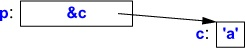
\includegraphics[scale=0.6]{img/015.jpg}
		\caption{Puntatore}
		\label{fig: 015}
	\end{center}
\end{figure}

La funzione fondamentale dei puntatori è quella dello scollegamento del riferimento ("dereferencing"), ovvero riferirsi ad un oggetto tramite il suo puntatore. Questa operazione è chiamata indirizzamento ("indirection"). L'operatore di dereferenziamento unario è *. Ad esempio:
\lstinputlisting[language=C++]{code/078.cpp}\label{code: 078}
L'oggetto puntato da p è c, e il valore di c è 'a', quindi il valore di *p assegnato a c2 è 'a'.

I puntatori puntano a unità di memoria minima, il valore più piccolo che possono puntare è un char (notare che i bool hanno la stessa grandezza minimo).

Se si volesse valutare a livello di bit si potrebbe usare un operatore bitwish, come vedremo poi, o un bitset.

Sfortunatamente puntatori ad array e puntatori a funzioni hanno una notazione più complicata:
\lstinputlisting[language=C++]{code/079.cpp}\label{code: 079}

\subsection{void*}
void* è un puntatore ad un oggetto di cui non si conosce la variabile restituita. Può essere usato solo per puntare a variabili, non a funzioni o ad un membro interno di una classe. In più void* può essere associato ad un altro void*, può essere usato per comparazioni e può essere convertito esplicitamente ad un altro tipo. Altre operazioni non sono sicure in quanto il compilatore non potrebbe sapere che variabile è puntata. Per poter usare un void* dobbiamo convertirlo esplicitamente ad un puntatore di un tipo conosciuto. Per esempio:
\lstinputlisting[language=C++]{code/080.cpp}\label{code: 080}

\subsection{nullptr}
nullptr rappresenta un puntatore a null, ovvero un puntatore che per ora inutilizzato. Può essere assegnato ad ogni puntatore ma non a tipi built-in:
\lstinputlisting[language=C++]{code/081.cpp}\label{code: 081}

\section{Array}
Per un tipo T, T[size] è un "array di size elementi di tipo T". Gli elementi sono indicizzati [0, size-1].

Si può accedere agli elementi dell'array con la notazione array[n] dove n è l'indice dell'elemento. Gli accessi out of bound sono pericolosi e soprattutto spesso non sono controllati.

Il numero di elementi deve essere un'espressione costante, ovvero o un valore fisso o il risultato di una constexpr.

Array multidimensionali possono essere espressi come array di array.

Se si ha visogno che i dati siano contigui un array è ideale, altrimenti può creare problemi.
\lstinputlisting[language=C++]{code/082.cpp}\label{code: 082}
Un array può essere allocato staticamente, sullo stack o nel free store:
\lstinputlisting[language=C++]{code/083.cpp}\label{code: 083}

Non esiste un assegnamento di un array e il nome di un array viene implicitamente convertito ad un puntatore verso il suo primo elemento.

In particolare, è meglio evitare di usare puntatori nelle interfacce perchè la loro conversione automatica a puntatori provoca molti problemi generalmente. Se si alloca un array sul free store allora ci si deve assicurare di usare delete[] sul suo puntatore solo dopo il suo ultimo utilizzo.

La maniera più sicura per avere un array sul free store è quello di avere un riferimento come una stringa, un vettore o un unique\_ptr. Se viene allocato staticamente allora bisogna essere sicuri di non cancellarlo mai.

Uno degli usi più comuni di un array terminato da 0 sono le stringhe in C. In C++ alcune librerie standard si basano su di ciò.

\subsection{Inizializzazione di array}
Un array può essere inizializzato con una serie di valori. Nel caso venga dichiarato così, la grandezza dell'array verrà adattata al numero di elementi della lista. Se invece viene esplicitata la dimensione e si eccede con i dati in ingresso allora ci sarà un errore. Se invece se ne danno meno ci sarà un padding di 0 nelle celle non esplicitate:
\lstinputlisting[language=C++]{code/084.cpp}\label{code: 084}
Non c'è una copia built-in per gli array. Non puoi inizializzare un array con un altro, nemmeno se dello stesso tipo, e non c'è un assegnamento di array.
\lstinputlisting[language=C++]{code/085.cpp}\label{code: 085}

Quando si ha bisogno di un assegnamento ad una collezione di oggetti, meglio usare un vettore, un array o un valarray.

\subsection{Stringhe}
Attenzione ad alcune peculiarità delle stringhe:
\begin{itemize}
	\item le stringhe generalmente vengono considerate come terminate da \textbackslash0, quindi nel caso sia presente uno \textbackslash0 a metà frase difficilmente il compilatore penserà che ci sia altro dopo.
	\item il compilatore considera un array di stringhe come una stringa continua
\end{itemize}

\subsubsection{Raw string}
In certi casi un backslash è solo un backslash \textst{e un sigaro è solo un sigaro}.

Per quei casi si può usare una raw string, indicata con un prefisso R alla dichiarazione della stringa:
\lstinputlisting[language=C++]{code/086.cpp}\label{code: 086}

E se volessi includere nella stringa "(? In questo caso possiamo usare un delimitatore interno alla stringa, l'importante è che sia simmetrico:
\lstinputlisting[language=C++]{code/087.cpp}\label{code: 087}

E le regex? Poter usare raw string in una regex è molto utile, soprattutto per casi complicati. In compenso non esistono caratteri di escape.

\subsubsection{Set di caratteri estesi}
Nel caso si abbia bisogno di caratteri speciali, si possono sfruttare le wchar\_t implicitamente:
\lstinputlisting[language=C++]{code/088.cpp}\label{code: 088}

\section{Puntatori negli array}
Il nome di un array può essere usato come puntatore per il primo elemento, ad esempio:
\lstinputlisting[language=C++]{code/089.cpp}\label{code: 089}
\begin{figure}[h!]
	\begin{center}
		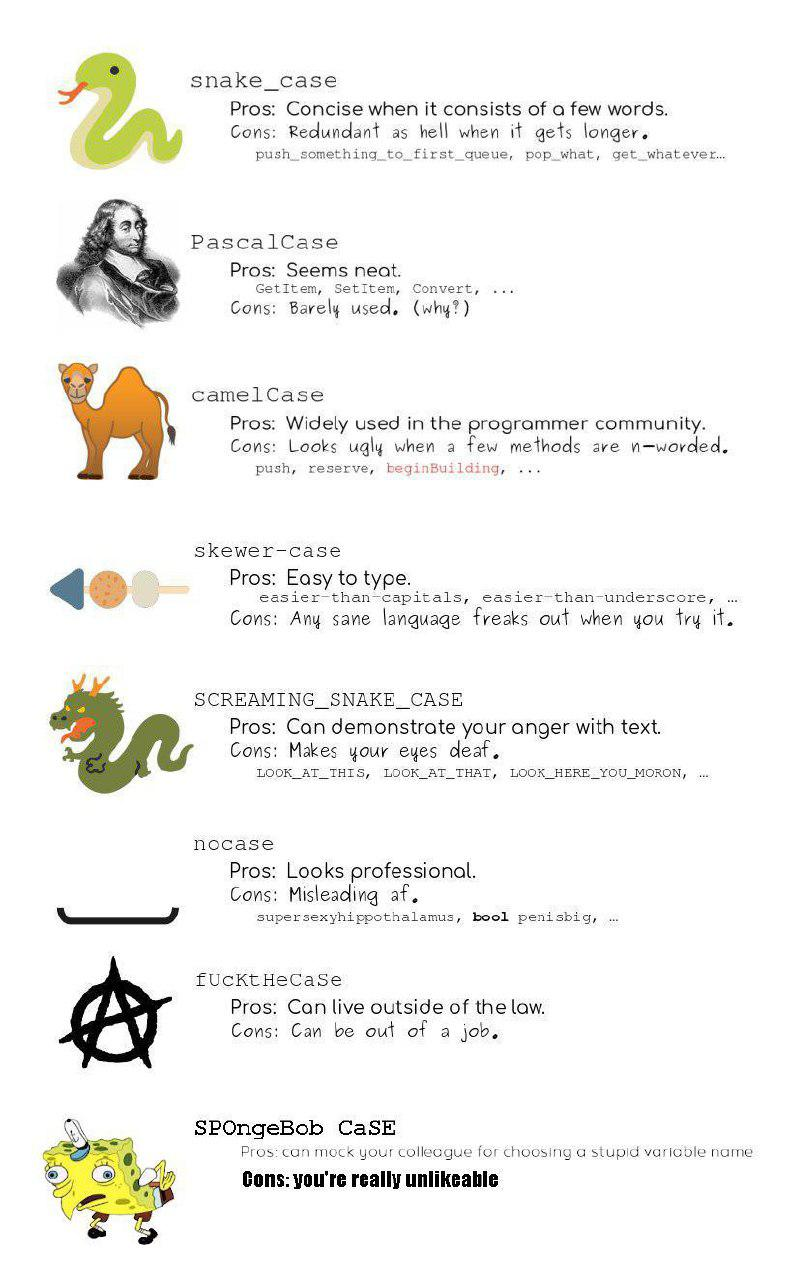
\includegraphics[scale=0.6]{img/016.jpg}
		\caption{Puntatori negli array}
		\label{fig: 016}
	\end{center}
\end{figure}

Mai puntare a prima o dopo l'array.

La conversione implicita di un array al suo puntatore significa che la dimensione dell'array si perde. Proprio per questo motivo è preferibile usare \emph{vector}, \emph{array} e \emph{string} della libreria standard, perchè superano questa difficoltà con \emph{size()}.

\subsection{Navigare tra gli array}
Si può accedere ad un array in due modi:
\begin{enumerate}
	\item direttamente iterando su di esso
	\item sfruttando i puntatori
\end{enumerate}
\lstinputlisting[language=C++]{code/090.cpp}\label{code: 090}
Il prefisso * dereferenzia un puntatore, in questo modo *p è il carattere puntato da p e ++ incrementa il puntatore. Le due versioni sono identiche per il compilatore.

Per ogni array a e intero j, dove j è interno al range di a:
\lstinputlisting[language=C++]{code/091.cpp}\label{code: 091}

\subsection{Passare un array}
Gli array non vengono passati per valore ma per puntatore al primo elemento.
\lstinputlisting[language=C++]{code/092.cpp}\label{code: 092}
A cosa può portare questo? Che gli array vengano passati per valore e non per indirizzo alle funzioni, rischiando di creare effetti collaterali.

\section{Puntatori e costanti}
C++ offre due significati a costante:
\begin{itemize}
	\item \emph{constexpr}: valutata durante la compilazione
	\item \emph{const}: non modificata all'interno dello scope
\end{itemize}

Il ruolo di \emph{consexpr} è di garantire la valutazione a compilazione, mentre \emph{const} è di essere immutabile per le interfacce.

Le costanti hanno una grande utilità, in più bisogna tenere conto del fatto che:
\begin{itemize}
	\item Avere delle costanti simboliche invece di stringhe all'interno del codice è spesso utile
	\item Molti puntatori vengono spesso letti ma non scritti
	\item In molte funzioni i parametri vengono letti ma non scritti
\end{itemize}

Poichè una costante non può essere mutata deve essere inizializzata durante la sua dichiarazione.
\lstinputlisting[language=C++]{code/094.cpp}\label{code: 094}
Quando viene usato un puntatore, due oggetti sono coivolti: il puntatore e l'oggetto a cui punta. Mettere come prefisso di un puntatore \emph{const} rende l'oggetto, ma non il puntatore, una costante. Per dichiarare un puntatore costante dobbiamo usare *const invece del solo *. Ad esempio:
\lstinputlisting[language=C++]{code/093.cpp}\label{code: 093}
Un modo per capire meglio questa scrittura è leggere da destra a sinistra, ad esempio "cp è una costante puntatore a un char" e "pc2 è un puntatore ad un char costante"

Un oggetto che è costante quando viene acceduto tramite un puntatore potrebbe essere variabile quando acceduto tramite altre vie. Dichiarando un puntatore costante la funzione impedisce di modificare l'oggetto puntato. Per esempio:
\lstinputlisting[language=C++]{code/095.cpp}\label{code: 095}
La prima versione è usata per le strighe quando l'elemento non deve essere modificato e ritorna un puntatore ad una costante che non permette modifiche. La seconda versione è usata per stringhe modificabili.

\section{Riferimenti}
Un puntatore ci permette di passare anche grandi quantità di dati con il minimo sforzo. Il tipo di puntatore determina cosa si possa fare con i dati attraverso il puntatore. Usare un puntatore è differente dall'usare il nome di un oggetto in alcuni modi:
\begin{itemize}
	\item Possiamo usare una sintassi differente, ad esempio *p invece di obj e p->m invece di obj.m
	\item Possiamo creare un puntatore che punti a diversi oggetti in momenti differenti
	\item Dobbiamo essere attendi quando usiamo puntatori in quando un puntatore potrebbe essere nullptr o puntare ad un oggetto che non era quello che ci aspettavamo
\end{itemize}

Queste differenze possono essere pesanti, ad esempio il controllo che non punti a nullptr. Molti problemi possono essere risolti tramite riferimenti (reference) che sono alias per un oggetto, solitamente implementato per contenere l'indirizzo di un oggetto e non impongono overhead di prestazioni comparati ai puntatori.

Le differenze con i puntatori sono:
\begin{itemize}
	\item Puoi accedere ad un riferimento con esattamente la stessa sintassi del nome di un oggetto
	\item un riferimento si riferisce sempre all'oggetto con il quale è stato inizializzato
	\item non è un riferimento nullo e possiamo assumere che un riferimento si riferisca sempre ad un oggetto
\end{itemize}

\lstinputlisting[language=C++]{code/096.cpp}\label{code: 096}

L'idea di passare per riferimento un valore ad una funzione è vecchissima. Ci sono tre tipi di riferimenti:
\begin{enumerate}
	\item lvalue: si riferiscono ad oggetti che vogliamo cambiare
	\item const: si riferiscono ad oggetti immutabili
	\item rvalue: si riferiscono ad oggetti che non vogliamo preservare dopo l'uso
\end{enumerate}

\subsection{Riferimenti lvalue}
Nel tipo della variabile una notazione X\& significa "riferimento a X". É usata per riferirsi ad un lvalue
\lstinputlisting[language=C++]{code/097.cpp}\label{code: 097}

Per assicurare che il riferimento sia un nome di qualcosa dobbiamo inizializzare il riferimento
\lstinputlisting[language=C++]{code/098.cpp}\label{code: 098}

L'inizializzazione di un riferimento è differente dall'assegnamento. 
\lstinputlisting[language=C++]{code/099.cpp}\label{code: 099}
Qua ++rr non incrementa il riferimento di rr, è invece applicato all'intero al quale si riferisce rr, ovvero var. Conseguentemente il valore di un riferimento non può essere cambiato dopo l'inizializzazione. Per ottenere un puntatore ad un oggetto possiamo scrivere \&rr. Non possiamo avere un puntatore ad un riferimento.

Notare una cosa:
\lstinputlisting[language=C++]{code/100.cpp}\label{code: 100}

Risultato? Uguale. Leggibilità? Decisamente migliore quella di next. Tendenzialmente è meglio evitare funzioni che modifichino le variabili passate.

\subsection{Riferimenti rvalue}
L'idea di avere più di un tipo di reference è per supportare differenti tipi di uso degli oggetti:
\begin{itemize}
	\item un lvalue non costante si riferisce ad un oggetto sul quale l'utente può scrivere
	\item un lvalue costante è immutabile
	\item un rvalue si riferisce ad un oggetto temporaneo che l'utente può modificare, assunto che l'oggetto non verrà mai più usato
\end{itemize}

Il dichiaratore \&\& significa "riferimento a rvalue". Non usiamo const in questo caso. Molti dei benefici risultanti dall'usare un riferimento rvalue sono legati alla scrittura dell'oggetto al quale si riferiscono. Sia un lvalue costante che un rvalue possono essere legati ad un rvalue, ciò che cambia è lo scopo:
\begin{itemize}
	\item Possiamo usare un riferimento rvalue per implementare una lettura distruttiva per ottimizzare quello che altrimenti sarebbe una copia
	\item possiamo usare un riferimento ad un lvalue costante per prevenire modifiche degli argomenti
\end{itemize}

\subsection{Riferimenti a riferimenti}
Se si ha un riferimento ad riferimento si ottiene semplicemente un riferimento alla variabile del primo. Ma che tipo di riferimento?
\lstinputlisting[language=C++]{code/102.cpp}\label{code: 102}

In altre parole vince l'lvalue. 

I riferimenti a riferimenti possono accadere come risultato di un alias o di un argomento per un template.

\chapter{Strutture, unioni ed enumerazioni}
\begin{itemize}
	\item struct: sequenza di elementi di tipo arbitrario
	\item union: una struct che mantiene solo uno dei suoi elementi alla volta
	\item enum: set di nomi costante
	\item enum class: è una enum dove gli enumeratori sono all'interno dello scope dell'enumerazione e non ci sono conversioni implicite
\end{itemize}

\section{Strutture}
Un array è un'aggregazione di elementi dello stesso tipo. Nella sua forma più semplice, una \emph{struct} è un aggreato di elementi di tipo arbitrario. Ad esempio:
\lstinputlisting[language=C++]{code/103.cpp}\label{code: 103}
Ciò definisce un tipo chiamato Indirizzo, consistente degli oggetti di cui si ha bisogno per inviare mail a qualcuno all'interno degli Stati Uniti.

Le variabili di tipo Indirizzo possono essere dichiarate come ogni altra variabile, e i membri individuali possono essere acceduti tramite dot notation (\emph{struct.elemento}). Ad esempio:
\lstinputlisting[language=C++]{code/104.cpp}\label{code: 104}

notare che jd.state potrebbe non essere inizializzato dalla stringa "NJ". Le stringhe terminano con \textbackslash0m quindi "NJ" ha tre caratteri. Uno in più rispetto a quanto contenibile da jd.state.

Spesso le strutture sono accedute tramite puntatore usando l'operatore ->. Ad esempio>:
\lstinputlisting[language=C++]{code/105.cpp}\label{code: 105}

Quando p è un puntatore, p -> è equivalente e (*p).m

Alternativamente, una \emph{struct} può essere passata per riferimento e acceduta tramite .:
\lstinputlisting[language=C++]{code/106.cpp}\label{code: 106}

\subsection{Layout delle \emph{struct}}
Un oggetto di una \emph{struct} contiene i suoi membri nell'ordine di dichiarazione. Ciò può portare a un problema di allineamento (vedere pagina \pageref{par: Allineamento}).

\subsection{nomi delle \emph{struct}}
Il nome di una struct è subito utilizzabile tramite puntatore:
\lstinputlisting[language=C++]{code/107.cpp}\label{code: 107}

Mai istanziare direttamente una variabile dello stesso tipo:
\lstinputlisting[language=C++]{code/108.cpp}\label{code: 108}

Per permettere a due struct di fare riferimento a vicenda basta anche solo dichiararne il nome prima:
\lstinputlisting[language=C++]{code/109.cpp}\label{code: 109}

\subsection{Strutture e classi}
Una struct è semplicemente una classe dove i membri sono pubblici di default. Una struct quindi può avere funzioni e costruttori, ad esempio:
\lstinputlisting[language=C++]{code/110.cpp}\label{code: 110}

Non devi scrivere un costruttore solo per inizializzare le variabili, serve anche per ordinare gli argomenti, convalidarli, modificarli, stabilire invarianti, ecc.. Ad esempio:
\lstinputlisting[language=C++]{code/111.cpp}\label{code: 111}

\subsection{Equivalenza e struct}
Due struct sono differenti tipi che possono avere anche gli stessi elementi. Quindi l'uguaglianza o l'assegnamento tra struct diverse non restituisce niente.

\section{Unioni}
Una \emph{union} è un \emph{struct} nella quale tutti i membri sono allocati allo stesso indirizzo, in questo modo la \emph{union} oocupa sempre e solo tanto spazio quanto l'elemento più grande. Ovviamente, una \emph{union} può contenere un solo valore alla volta.
\lstinputlisting[language=C++]{code/112.cpp}\label{code: 112}
I membri s ed i non possono mai essere usati allo stesso momento, si potrebbe rimediare specificando che entrambi dovrebbero essere un'unione.
\lstinputlisting[language=C++]{code/113.cpp}\label{code: 113}
Il linguaggio non tiene traccia di quale valore è contenuto nella \emph{union}, quindi il programmatore deve fare ciò:
\lstinputlisting[language=C++]{code/114.cpp}\label{code: 114}

Per evitare errori, uno può incapsulare una \emph{union} in modo che la corrispondenza tra tipo e accesso all'unione possa essere garantita.

La \emph{union} può certe volte essere usata male per "conversione di tipi". Questo uso errato è praticato soprattutto da programmatori che sono esperti in linguaggi che non hanno una conversione esplicita, quindi devono barare. Ad esempio "convertire" int in int* può essere assunto tramite equivalenza bitwise:
\lstinputlisting[language=C++]{code/115.cpp}\label{code: 115}
Questa non è una conversione.
Le unioni possono essere essenziali da un punto di vista prestazionale. Bisogna tenere da conto che sono molto prone ad errori, quindi è meglio considerare di usarle il meno possibile.

\subsection{\emph{Union} e classi}
Tecnicamente, una \emph{union} è un tipo di \emph{struct} che è un tipo di classe. Le differenze sono:
\begin{itemize}
	\item una \emph{union} non può avere funzioni virtuali
	\item una \emph{union} non può avere membri che siano reference
	\item una \emph{union} non può avere una classe base
	\item una \emph{union} ha un membro con un costruttore definito dall'utente, un'operazione di copia, una di spostamento o un decostruttore, e offre una speciale funzione delete per l'unione
	\item al massimo un membro della \emph{union} può avere un inizializzaore
	\item una \emph{union} non può essere usata come classe base
\end{itemize}

\subsection{\emph{Union} anonime}
Per vedere come possiamo scrivere una classe che superi i problemi di una \emph{union} consideriamo una viariante di \emph{Entry}:
\lstinputlisting[language=C++]{code/116.cpp}\label{code: 116}

La funzione di accesso può essere definita come:
\lstinputlisting[language=C++]{code/117.cpp}\label{code: 117}

Queste funzioni controllano il tag \emph{type} e se una di queste corrisponde all'accesso desiderato, ritorna un riferimento al valore, altrimenti lancia un'eccezione. Una \emph{union} implementata così è chiamata \emph{tagged union} o \emph{discrimination union}.

Queste funzioni non prendono da conto come il nuovo valore dovrebbe prendere da conto anche il valore precedente:
\lstinputlisting[language=C++]{code/118.cpp}\label{code: 118}




\end{document}
